% Created 2021-04-20 Tue 13:36
% Intended LaTeX compiler: pdflatex
\documentclass[11pt]{article}
\usepackage[utf8]{inputenc}
\usepackage[T1]{fontenc}
\usepackage{graphicx}
\usepackage{grffile}
\usepackage{longtable}
\usepackage{wrapfig}
\usepackage{rotating}
\usepackage[normalem]{ulem}
\usepackage{amsmath}
\usepackage{textcomp}
\usepackage{amssymb}
\usepackage{capt-of}
\usepackage{hyperref}
\usepackage[margin=0.5in]{geometry}
\author{Fabio Favero Henkes}
\date{\today}
\title{}
\hypersetup{
 pdfauthor={Fabio Favero Henkes},
 pdftitle={},
 pdfkeywords={},
 pdfsubject={},
 pdfcreator={Emacs 26.1 (Org mode 9.1.9)},
 pdflang={English}}
\begin{document}

\tableofcontents


\section{Star Wars Rebellion}
\label{sec:org12d429a}

\subsection{Fase de Atribuição}
\label{sec:orgcca3c0c}

Atribuir líderes à missões.

\begin{center}
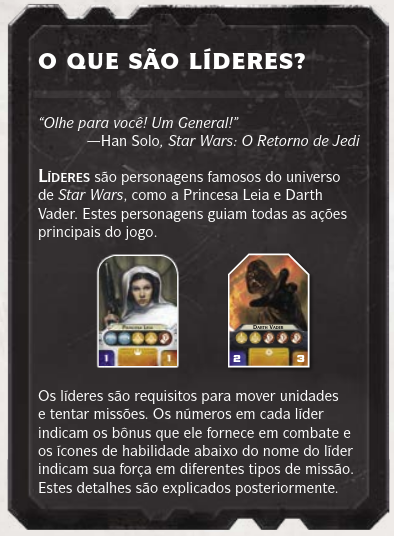
\includegraphics[width=2.0in]{./lider.png}
\end{center}

O jogador Rebelde começa atribuindo seus líderes a missões. Quando terminar, o jogador Imperial atribui seus líderes a missões.

Cada missão possui um requisito de habilidade no canto superior esquerdo.

\begin{center}
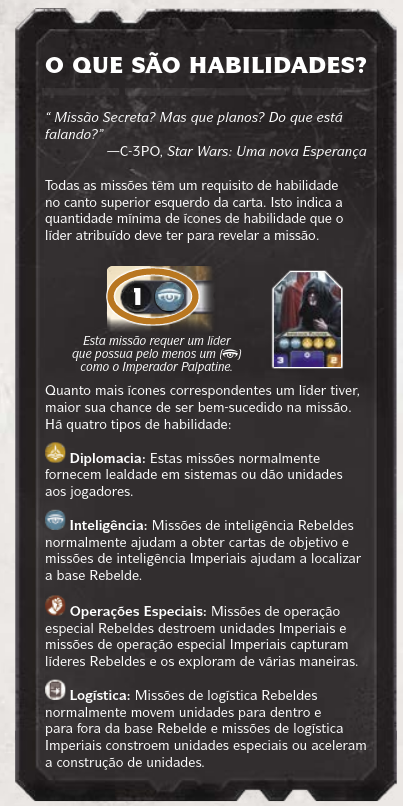
\includegraphics[width=2.0in]{./skills.png}
\end{center}

\subsection{Fase de Comando}
\label{sec:orgb0a1e2b}

\begin{itemize}
\item \textbf{Ativar um Sistema}:
\end{itemize}

Use um líder de sua reserva de líderes para mover unidades no tabuleiro e possivelmente iniciar um combate.

Unidades terrestres e TIE fighters precisam ser transportados (verifique a capacidade da nave de transporte).

\begin{itemize}
\item \textbf{Revelar uma Missão}:
\end{itemize}

Use um líder em uma carta de missão para revelar o efeito da carta.

\begin{center}
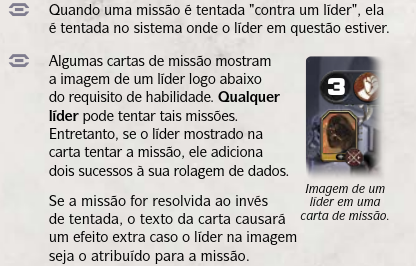
\includegraphics[width=2.0in]{./lider-effect.png}
\end{center}

O termo \textbf{RESOLVA} significa que o efeito da carta acontece automaticamente e não pode ser contraposto.

O termo \textbf{TENTE} significa que o efeito da carta só acontece se a missão for bem-sucedida. A missão é considerada automaticamente bem-sucedida a menos que seja contraposta por um líder adversário.

Para \textbf{CONTRAPOR} uma missão seu adversário pode escolher um líder de sua reserva para contrapor essa missão. Um líder adversário é colocado no mesmo sistema onde a missão está sendo tentada.

Se ambos jogadores tiverem um líder no sistema, a missão é considerada contraposta.

Os jogadores rolam dados (de qualquer cor) igual a soma dos ícones de habilidade de todos os seus líderes nesse sistema.

Os dados são rolados somente para ícones correspondentes ao requisito de habilidade da missão.

\subsection{Fase de Restauração}
\label{sec:orgf2d30bf}

\begin{itemize}
\item \textbf{Retornar líderes}:
\end{itemize}

Os líderes são retornados à reserva. Caso ainda estejam sobre alguma carta de missão, esta volta para a mão.

\begin{itemize}
\item \textbf{Comprar missões}:
\end{itemize}

Cada jogador compra duas cartas, caso possua mais de 10 cartas, descarta até o limite.

\begin{itemize}
\item \textbf{Lançar sondas}:
\end{itemize}

O jogador Imperial compra duas cartas de sonda. Cada carta de sonda mostraum sistema onde a base Rebelde \textbf{NÃO} está localizada. O jogador Imperial mantém estas cartas em segredo.

\begin{itemize}
\item \textbf{Comprar objetivo}:
\end{itemize}

O jogador Rebelde compra uma carta de objetivo.

\begin{itemize}
\item \textbf{Avançar marcador de tempo}:
\end{itemize}

Avance o marcador de tempo um espaço no indicador.

\begin{center}
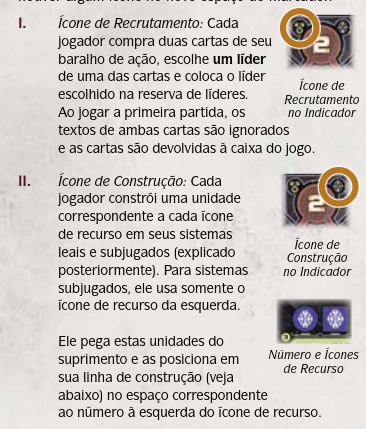
\includegraphics[width=2.0in]{./time-marker.png}
\end{center}

\begin{itemize}
\item \textbf{Destacar unidades}:
\end{itemize}

Cada jogador desliza todas as suas unidades um espaço para baixo em sua linha de construção

Unidades que deslizarem para fora do espaço "1" estão prontas para serem usadas.

O jogador posiciona essas unidades em sistemas onde possui marcadores de lealdade ou subjugação.

Cada jogador pode destacar no máximo duas unidades em cada sistema.

\subsection{Vencendo o jogo}
\label{sec:org797c10e}

O jogador Imperial vence se encontrar e destruir a base rebelde. Se o jogador Imperial possuir lealdade ou unidades terrestres no mesmo sistema da base Rebelde, a base Rebelde é revelada imediatamente.

O jogador Rebelde vence se o marcador de turno encontrar o marcador de reputação.

O marcador de reputação (com o ícone dos Rebeldes) sobe o valor determinado na carta de objetivo quando este objetivo é cumprido.

O jogador Rebelde pode jogar a carta de objetivo de sua mão se a tiver completado o requisito da carta no momento especificado.

\begin{itemize}
\item \textbf{Regras adicionais:}
\end{itemize}

\begin{center}
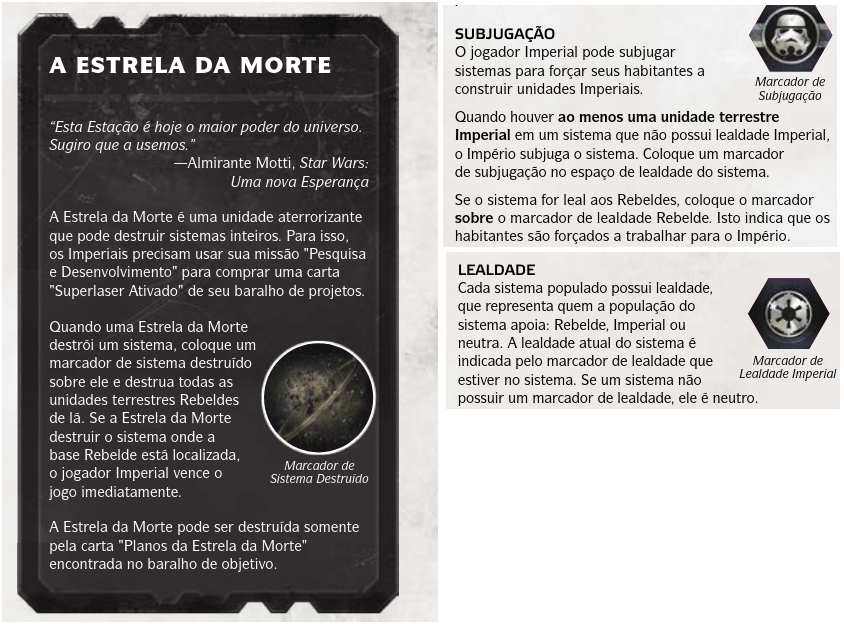
\includegraphics[width=4.0in]{./details.png}
\end{center}
\end{document}
